% Shortened final report (2 pages + references), ACL style.
% Cut from reports/final/main.tex: Related Work, the overview, degree and
% held out figures, the expectations table and the implementation detail.
% Compile: pdflatex main && bibtex main && pdflatex main && pdflatex main
\documentclass[11pt]{article}

\usepackage[final]{acl}

\usepackage{times}
\usepackage{latexsym}
\usepackage[T1]{fontenc}
\usepackage[utf8]{inputenc}
\usepackage{microtype}
\usepackage{inconsolata}
\usepackage{amsmath}
\usepackage{amssymb}
\usepackage{booktabs}
\usepackage{graphicx}

\newcommand{\action}[1]{\texttt{#1}}
\newcommand{\seed}{S_i^{(0)}}

\title{When does graph expansion help? Measurement-Driven, Issue-Adaptive\\
Retrieval Routing for Repository-Level Code Localization}

\author{
  Naman Singhal \\
  2024114013 \\
  \And
  Yash More \\
  2024114004 \\
  \And
  Aaditya Bhatia \\
  2023114012
  % Project links
  \AND
  \normalfont\small Code: \url{https://github.com/the-neemon/adaptive-code-localization} \\
  \normalfont\small Video: \url{https://drive.google.com/file/d/1_9jMnOhiX369Kbzup602AR-bN0CjNckm/view?usp=sharing}
}

\raggedbottom
\begin{document}
\maketitle

\begin{abstract}
Graph-based coding agents follow calls, imports and inheritance to find the
code an issue needs, but leave the decision of when to expand to the model.
We measure that decision directly. On the 500 Python issues of SWE-Explore,
we run six retrieval actions post BM25 seed under a fixed line budget.
Graph expansion helps about 40\% of issues and hurts about 40\%, so picking
the best action per issue would score 40\% above the best fixed action, yet
cheap signals predict little of this. A rule-based router tested on held-out
repositories closes about 5\% of that gap (interval includes zero) and its
single stable rule about 7\%; a classifier router does not beat the best
fixed action.
\end{abstract}

\section{Introduction}

Before a coding agent can fix an issue, it must find the relevant code under a
hard context budget whereby every retrieved chunk displaces another. Lexical
(BM25; \citealp{robertson2009bm25}) and dense retrievers are cheap but miss
code only reachable via program structure. Graph-based agents such as
LocAgent~\citep{chen2025locagent}, CoSIL~\citep{jiang2025cosil} and
OrcaLoca~\citep{yu2025orcaloca} traverse a repository graph, but decide
where to expand within the model. We ask (Phase~A) what each retrieval action
is worth over a BM25 seed for each issue under a fixed budget, and which cheap
signals predict it, and (Phase~B) whether an explicit router built from these
findings beats the best fixed action on repositories it has never seen.

\section{Method and Setup}

\paragraph{Data.} SWE-Explore~\citep{zhang2026sweexplore} builds ground truth
from the code successful agent trajectories read: core regions (the code the
trajectories agree on) and optional ones (read by only some). Joined with
SWE-bench Verified~\citep{jimenez2024swebench} and SWE-bench Pro, its Python
subset is 500 issues from 15 repositories (Django alone has 207).

\paragraph{Actions.} Every system returns ranked code chunks (functions,
class bodies, module-level code) from the pre-fix snapshot, cut to $B$ lines
($B=300$ primary), so no action can win by returning more code. The seed
$\seed$ is BM25 over chunks. \action{stop} keeps it; \action{dense} uses the
frozen CodeRankEmbed encoder~\citep{suresh2025cornstack}; \action{fusion} is
reciprocal-rank fusion~\citep{cormack2009rrf} of the two; and
\action{expand}$(e)$ scores each depth-1 neighbour $n$ of the top 10 seed
chunks along calls, imports or inheritance as
$\max\big(s(n), \lambda \max_p s(p)\big)$. The gain of action $a$ is
$\Delta(i,a) = \mathrm{nDCG}(S_i^{(a)}) - \mathrm{nDCG}(\seed)$; the oracle
picks the best action per issue in hindsight.

\paragraph{Routers and splits.} Routers use 16 cheap features available after
the seed (e.g.\ traceback present, file named, BM25 score margins, graph
degree of the top hit, BM25/dense overlap). Tier~1 is an ordered rule list
built by a fixed greedy procedure (default: the best fixed action; at most 5
rules, each with a positive repository-bootstrap lower bound); Tier~2 is a
classifier. A dev set of 3 repositories (56 issues) is used only for tuning;
the other 444 issues form 8 leave-one-repository-out folds. Intervals are
95\% repository-clustered bootstrap intervals.

\paragraph{Benchmark findings.} The released SWE-Explore scorer normalizes
nDCG by the best reordering of the system's own output, unlike the paper's
ground-truth ideal: 75 of the 500 BM25 seeds get a perfect official nDCG@300
while covering 14\% of the core lines. We use the paper's definition. The
ground truth is mostly whole files, so even a perfect ranker reaches only
39.5\% line recall at $B=300$.

\section{Phase A: The Value of Each Action}

\begin{table}[t]
\centering
\small
\setlength{\tabcolsep}{4pt}
\begin{tabular}{@{}l ccc cc@{}}
\toprule
 & \multicolumn{3}{c}{nDCG@$B$} & Rec. & File \\
\cmidrule(lr){2-4}
Action & 100 & 300 & 500 & @300 & @300 \\
\midrule
\action{stop} (seed)      & .264 & .172 & .144 & .120 & .628 \\
\action{expand(inherit)}  & .264 & .172 & .144 & .120 & .638 \\
\action{expand(imports)}  & .263 & .170 & .143 & .131 & .596 \\
\action{expand(calls)}    & .280 & .178 & .146 & .127 & .646 \\
\action{dense}            & .213 & .152 & .128 & .128 & .676 \\
\action{fusion}           & .268 & .184 & .156 & .136 & .706 \\
\midrule
Oracle                    & .392 & .258 & .212 & & \\
\bottomrule
\end{tabular}
\caption{Phase A means over 500 issues. Rec.: line recall. File: share of
the developer patch's files that came back (410 SWE-bench Verified issues).}
\label{tab:main}
\end{table}

\begin{figure}[t]
\centering
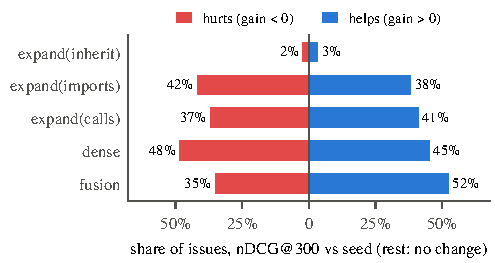
\includegraphics[width=\columnwidth]{figures/helps_hurts.pdf}
\caption{Share of issues each action helps or hurts compared with the seed
(nDCG@300, 500 issues).}
\label{fig:helps}
\end{figure}

At $B=300$ only fusion reliably beats the seed on average ($+0.012$,
$[+0.002, +0.031]$), only dense is reliably worse, and no graph expansion
moves the average (Table~\ref{tab:main}). Per issue, though, every action
except \action{expand(inherit)} helps 38 to 52\% of issues and hurts another
35 to 48\% (Figure~\ref{fig:helps}). The oracle scores 0.258 against
fusion's 0.184, 40\% higher, with its choice spread evenly across five
actions.

\paragraph{Which signals predict the gain?} Of the five expectations in our
proposal (traceback $\rightarrow$ call expansion helps, named target file
$\rightarrow$ expansion adds noise, hub top hit $\rightarrow$ expansion
floods the budget, BM25/dense disagreement $\rightarrow$ fusion,
concentrated seed $\rightarrow$ stop), only the hub one holds, and only as a
contrast: call expansion gains 0.017 $[+0.009, +0.031]$ with a weakly
connected top hit (degree $\leq 4$). The strongest signal, which we did not
predict, is the graph degree of the top seed hit: with a hub (degree $>10$)
dense loses 0.062 $[-0.110, -0.036]$, and with a weakly connected one fusion
gains 0.040 $[+0.022, +0.080]$. Across feature bins, 46 of 205 cells exclude
zero against about 10 expected by chance: real but a very weak structure.

\section{Phase B: Routing on Held-Out Repositories}

\begin{table}[t]
\centering
\small
\setlength{\tabcolsep}{3pt}
\begin{tabular}{@{}lcccc@{}}
\toprule
System & nDCG & vs fixed & GapCl. & helps/hurts \\
\midrule
\action{stop} & .179 & & & \\
fixed (fusion) & .187 & & & \\
Tier 1 router & .191 & $+.004$ & $+.047$ & 17\% / 18\% \\
Tier 1, rule 1 & .193 & $+.006$ & $+.073$ & 7\% / 6\% \\
Tier 2 & .180 & $-.007$ & $-.099$ & 32\% / 39\% \\
oracle & .262 & & & \\
\bottomrule
\end{tabular}
\caption{Routers on the 444 held-out issues, nDCG@300. GapCl.\ (GapClosed):
share of the fixed-to-oracle gap closed. Gain intervals: Tier~1
$[-.004, +.009]$, rule 1 $[-.001, +.008]$, Tier 2 $[-.026, +.001]$.}
\label{tab:heldout}
\end{table}

For each fold the router is fit on all other issues and routes the held-out
repository; the procedure was fixed prior to any held-out result even existing.
Neither router reliably beats the best fixed action
(Table~\ref{tab:heldout}). Tier~1's first rule is the one stable finding: it
sends issues whose top hit has more than 7 call edges and whose BM25/dense
overlap is at most 0.2 to \action{expand(calls)}, and is chosen in all 8
folds (every other rule in at most 4). On its 64 issues dense scores 0.121
and fusion 0.161, while \action{expand(calls)} scores 0.213: dense is wrong
and fusion inherits its mistakes. Cut after this rule, the router closes
about 7\% of the gap. The Tier~2 classifier is reliably worse than the
one-rule router ($-0.013$, $[-0.026, -0.006]$), as it overfits 56 dev
issues. On SWE-bench Verified file recall (464 issues), fusion recovers 0.708
of the patched files and the Tier~1 router 0.690.

\section{Discussion and Conclusion}

The right action depends on the issue, and a per-issue oracle beats the best
fixed action by 40\%, but cheap post-seed signals capture little of this gap:
One rule carries across repositories and a learned classifier finds less.
This is the partly negative outcome that our proposal was expecting. Limitations:
15 repositories (41\% django) make intervals wide; the ground truth records
what agents read, often whole files; and we cover only Python, one dense
model and depth-1 expansion. A useful router will need richer signals than
those available right after a lexical first pass.

\bibliography{references}

\end{document}
